\documentclass[main]{subfiles}
\begin{document}

%@@@@@@@@@@@@@@@@@@@@@@@@@@@@@@
% summarizes lecture 11NN
% author: Joachim
%This is all copy pasta without any references. It is not intended to be published and/or distributed in any way! It is for our internal student group use only!

\section{Neural Networks}
This is the chapter on Neural Networks.
\subsection{Motivation by Computational Neuroscience}
Artificial neural networks are inspired by biology. In the human brain we have $10^{11}$ neurons with on average $10^{14}$ synapses, hence a extremely complex computational network.
The network is made of over 1000 different cell types. Neurons can act onto each other either in an excitatory or inhibitory fashion.

\subsection{Multilayer Perceptrons and Backpropagation}
\todo{Introduction,Layer counting/indexing problem}



\subsubsection{Training}
MLP training consists of these steps
\begin{enumerate}
\item Feed-forward input data to compute output
\item Compute misclassification error
\item Backpropagate error signal and alter weights



\end{enumerate}
\begin{figure}[H]
\centering
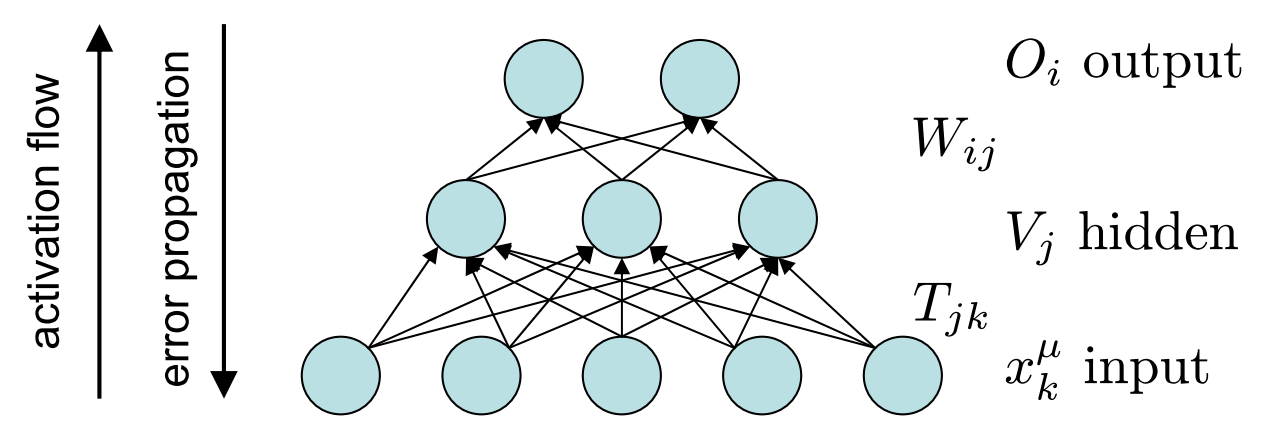
\includegraphics[width=0.7\linewidth]{figs/NN_Data_Flow}
\caption{Two layer MLP (input is not counted in modern nomenclature)}
\end{figure}


\subsubsection{Feed Forward}
The data is fed into layer 0 (also called input layer).
The sample (with index $\mu$)   has the form:
\begin{equation}
(x^{\mu},y^{\mu}),  1 \leq \mu \leq n
\end{equation}
At each node $V_j$ of the first Layer, all the inputs times the weight are summed up, giving us the activation of that node:
\begin{equation}
h_j^{\mu}=\sum_k T_{jk}x_k^{\mu}
\end{equation}
Where k is the index of the input/feature
This activation is then transformed using a nonlinear activation function to give
\begin{equation}
V_j^{\mu}=S(h_j^{\mu})=S(\sum_k T_{jk}x_k^{\mu})
\end{equation}
which will act as input for the next layer O. This layer, which in this example is also the output layer, performs again a summation followed by a transformation
\begin{equation}
O_i^{\mu}=S(\sum_j W_{ij}V_j^{\mu})=S(\sum_j W_{ij}S(\sum_k T_{jk}x_k^{\mu}))
\end{equation}
Where i is the index of the output node

\subsubsection{Error function}
\begin{equation}
J(W,T)=\frac{1}{2}\sum_{i,\mu}(y_i^{\mu}-S(\sum_j W_{ij}S(\sum_k T_{jk}x_k^{\mu})))^2=\frac{1}{2}\sum_{i,\mu}(y_i^{\mu}-O_i^{\mu})^2
\end{equation}

\subsubsection{Backpropagation}
There is no way to directly alter weights from all layers based on classification error. We have to propagate the error signal back from the output to the input layer. We use the chain rule to “assign the credit” (blame) for a
particular error to specific weights.
We start with the connections from the hidden layer to the output, hence the weights $W_{ij}$:

\begin{equation}
S'(x) = \frac{dS}{dx}
\end{equation}

\begin{equation}
\Delta W_{ij}= -\eta \frac{\partial J}{\partial W_{ij}}=\eta \sum_{\mu}(y_i^{\mu}-O_i^{\mu}) \cdot S'(\sum_l W_{il}V_l^{\mu}) \cdot V_j^{\mu}=\eta \sum_{\mu} \delta_i^{\mu}V_j^{\mu}
\end{equation}

where
\begin{equation}
\delta _i^{ \mu } \equiv S'( \sum_l W_{il}V_l^{ \mu })(y_i^{ \mu }-O_i^{ \mu })
\end{equation}

Next, we adapt the connections between input and hidden layer:
\begin{align*}
\Delta T_{jk}&=-\eta \frac{\partial J}{\partial T_{jk}}=-\eta \frac{\partial J}{\partial V_j^{\mu}}\frac{\partial V_j^{\mu}}{\partial T_{jk}}\\&=\eta \sum_{\mu i}(y_i^{\mu}-O_i^{\mu}) \cdot S'(\sum_l W_{il}V_l^{\mu})W_{ij}S'(\sum_l T_{jl}x_l^{\mu}) \\&=\eta \sum_{\mu i}\delta_i^{\mu}W_{ij}S'(\sum_l T_{jl}x_l^{\mu})x_k^{\mu} \\&=\eta \sum_{\mu}\tilde \delta_j^{\mu}x_k^{\mu}
\end{align*}

where
\begin{equation}
\tilde \delta_j^{\mu} \equiv S'(\sum_l T_{jl}x_l^{\mu})\sum_l W_lj \delta_l^{\mu}
\end{equation}

This leads to the \textbf{General learning rule:}
\begin{equation}
\Delta W_pq=\eta \sum_{\textnormal{patterns}} \delta_{\textnormal{output}} V_{\textnormal{input}}
\end{equation}

\textbf{Backpropagation Algorithm}
\begin{enumerate}
\item Initialize the weights $W^m_{ij}$ with small random values
\item  Choose a pattern $x^{\mu}_k$ and feed it to the input layer $(m = 0)$, i.e., $V^0_k= x^{\mu}_k, \forall k$
\item  Propagate the activity through the network where $V_i^m=S(\sum_j W_{ij}^mV_j^{m-1})$ holds for each $i$ and each layer m
\item   Calculate the weight corrections for the output layer $\delta_i^M=S'(h_i^M)[y_i^{\mu}-V_i^M]$ by comparing the actual output $V^M_i$ with the desired output $y^{\mu}_i$ for pattern $\mu$
\item  Calculate the weight corrections for the previous layers by sending back the error signal\\ $\delta_i^{m-1}=S'(h_i^{m-1})\sum_j W_{ji}^m \delta_j^m$ for $m = M, M-1, . . . , 2$, until a weight correction has been calculated for each unit.
\item  Use $\Delta W_{ij} = \eta \delta_i^mV_j^{m-1}$, to adapt all weights according to $W_{ij}^{\textnormal{new}}=W_{ij}^{\textnormal{old}}+\Delta W_{ij}$
\item   Goto 2 and repeat the loop for the next pattern
\end{enumerate}
\textbf{Remarks}
\begin{itemize}
\item \textbf{A perceptron with one inner layer can approximate every continuous function}
\item The weights should be initialized with small randon values close to zero: random initialization performs symmetry breaking,
bigger values generates flat spots.
\item The weights should not be initialized all as the same value: because this make all your activation units compute the same feature and
then, you network learns nothing.
\item Backpropagation can be implemented with online or iterative and with batch learning mode \\$\Delta W_{pq}=\eta\delta_{\textnormal{output}}^{\mu}V_{\textnormal{input}}^{\mu}$
\item Patterns should be presented in random order
\item Learning is sometimes accelerated by adding noise
\item The learning rule is local; all information after propagating back the error signal is available at node $i$
\item The learning rule lacks biological plausibility!
\item Rule of thumb: 5-10 training examples per independent weight are necessary


\end{itemize}

\textbf{Variations on Backpropagation}
\begin{itemize}
\item Alternative Cost Function \begin{itemize}[label={$\circ$}]
\item $J=\sum_{i,\mu}[y^{\mu}_ilog\frac{y_i^{\mu}}{O_i^{\mu}}+(1-y_i^{\mu})log\frac{1-y_i^{\mu}}{1-O_i^{\mu}}]$
\item $O_i^{\mu}$ is the probability that the hypothesis represented by a neuron is true
\item $y_i^{\mu}$ is the probability which is supposed to be learned
\end{itemize}
\item Convergence speedup by using momentum value \begin{itemize}[label={$\circ$}]\item $m \in \mathbb{R}^+$ , e.g. $m = 0.1$ \item
$\delta_i^{\mu}=(S'(\sum_lW_{il}V_l^{\mu})+m)(y_i^{\mu}-O_i^{\mu})$\end{itemize}
\item Alternative minimization techniques \begin{itemize}[label={$\circ$}]
\item Conjugate gradient methods
\item Methods based on the Hessian $\frac{\partial^2J}{\partial W^2_{ik}}$
\end{itemize}
\item Regularisation techniques to avoid overfitting
\begin{itemize}[label={$\circ$}]
\item Weight decay: rarely used weights decay to zero \\$J=J_0+\gamma\sum_{i,k}\frac{W_{i,k}^2}{1+W_{i,k}^2}$
\item Connections between neurons that strongly fluctuate during training are selectively eliminated
\end{itemize}

\end{itemize}

\subsection{Deep Neural Networks}
\subsubsection{Training Deep Networks}
\begin{itemize}
\item This learning rule minimizes the cost function
\begin{equation}
R=\sum_{\textnormal{visible nodes}}^{}Q_{\alpha}log \frac{Q_{\alpha}}{P_{\alpha}}(\{ w_{ik}\}) \textnormal{\space since \space} \Delta w_{ik}=-\eta \frac{\partial R}{\partial w_{ik}}
\end{equation}
The target probability and the derived probability of visible units are denoted by $Q_{\alpha}$ and $P_{\alpha}(\{w_{ik} \})$, respectively
\item Calculation of averages: Monte-Carlo simulation of a network. Disadvantage: training of a Boltzmann machine is rather
time consuming.

\end{itemize}


\subsection{Universal Approximation}
\textbf{Given:}\\ \begin{itemize}
\item function $f: \mathbb{R}^n \to \mathbb{R}^p$ to be learned
\item  $n$ input neurons, $p$ output neurons
\end{itemize}
\textbf{Prove}
\begin{itemize}
\item uniform approximation of $f$ on a compact support $\mathcal{K} \subset \mathbb{R}^n$
\item $\forall \epsilon  >0 \exists g \in \mathcal{G} $ such that $\lVert f(x)-g(x) \rVert<\epsilon$ \space\space $\forall x \in \mathcal{K}$
\end{itemize}
\textbf{Theorem}
\begin{itemize}
\item Every continuous function $f: \mathbb{R}^n \to \mathbb{R}^p$ can be uniformly approximated on the compact support K
by functions\\
$y_k=S_k(\alpha_k+\sum_{j\to k}w_{jk}S_j(\alpha_j+\sum_{i\to j}w_{ij}x_i))$, $S_k \in \mathcal{N}\mathcal{N}$\\
with linear output units and logistic $S(x)=\frac{1}{1+e^{-x}}$ hidden units
\item The notation $i \to j$ denotes the set of all
indices $i$, where the associated node has an edge to $j$
\end{itemize}


\subsection{Autoassociation}
XOR

%\subsection{NETtalk and ALVINN} Just Examples
\subsection{Boltzmann machines}
A Boltzmann machine, like a Hopfield network, is a network of units with an "energy" defined for the network. It also has binary units, but unlike Hopfield nets, Boltzmann machine units are stochastic.\\ %Wikipedia
Difference to MLP: The multilayer perceptron is a network with a purely feedforward dynamics, meaning the activity is propagated from layer $i$ to layer $i + 1$ without feedback. However, a Boltzmann machine is a type of stochastic recurrent neural network.\\
The states of the units/neurons are updated in an asynchronous stochastic way by using the Metropolis sampler.\\
\textbf{Dynamics}
\begin{itemize}
\item stochastic binary neurons $x_i \in \{0,1\}$ $1 \leq i \leq n$
\item asynchronous update rule $x_i^{(t+1)}=\left\{
  \begin{array}{ll}
    1 & \textnormal{if\space}\sum_{j=1}^n w_{ij}x_j^{(t)}\ge \theta_i\\
    0 & \textnormal{otherwise}
  \end{array}
\right.$

\end{itemize}

\subsubsection{Network Architecture}
\textbf{symmetric couplings}
\begin{itemize}
\item  $w_{ik} = w_{ik}$ $\Rightarrow$ cost function exists
\item $w_{ii}=0$\space\space$ \forall i$ (No unit has a connection with itself)

\end{itemize}
\textbf{costs of the network}
\begin{equation}
R(\{x_i\})=-\frac{1}{2}\sum_{i,k=1}^nw_{ik}x_ix_k+\sum_{i=1}^n\theta_ix_i
\end{equation}
The cost function $R(\{x^{(t)}_i\})$ is non-increasing under the deterministic asynchronous update rule:
\begin{equation}
x_i^{(t+1)}=\left\{
  \begin{array}{ll}
    1 & \textnormal{if\space}\sum_{j=1}^n w_{ij}x_j^{(t)}\ge \theta_i\\
    0 & \textnormal{otherwise}
  \end{array}
\right.
\end{equation}
Since $R(\{x^{(t)}_i\})$ is bounded from below for bounded weights $w_{ik}$ the update dynamics terminates with probability 1 after a finite number of steps.\\
\textbf{averages are calculated according to the Gibbs distribution}\\
\begin{equation}
\mathbb{E}[f]=\sum_{\{x_i\}}P(\{x_i\})f(\{x_i\})
\end{equation}with
\begin{equation}
P(\{x_i\})=\frac{exp(-R(\{x_i\})/T)}{\sum_{\{x_i\}}exp(-R(\{x_i\})/T)}
\end{equation}
Where $\sum_{\{x_i\}}$ denotes a sum over all possible $2^n$ configurations of the activities $x_i \in \{0, 1\}$

\subsubsection{Metropolis Sampler for Boltzmann Machines}
\textbf{MCMC Algorithm: (sequential asynchronous update)}\\
\begin{tabular}{ll}
    Input: & $n$ neurons, cost function $R(\{x_i \})$\\
    Output: & activity pattern $x : \{\textnormal{neurons}\} \to \{\textnormal{activities} \}$
  \end{tabular}
\begin{enumerate}
\item initialize $x(i) \in \{0, 1\}$ randomly; $t \gets 0$
\item repeat
\setlength{\itemindent}{.5in}
\item \indent $t \gets t+1$
\item \indent draw $x' \sim Q(x)$\space\space (where $Q(x)$ is the proposal distribution)
\item \indent $p \gets min\{exp(-(R(x')-R(x))/T),1\}$
\item \indent draw $b \sim$Bernoulli$(p)$
\item \indent if $b=1$ then $x \gets x'$
\setlength{\itemindent}{0in}
\item  until convergence
\end{enumerate}

\textbf{Variants}
Gibbs or importance sampling is competitive!(The Metropolis sampler is often used to calculate averages)

\subsubsection{Training of a Boltzmann Machine}
\begin{itemize}
\item let the network evolve under two different conditions \begin{enumerate}
\item clamped dynamics: fix the activity of the visible nodes to the input/output patterns and measure correlation differences in the activity of two nodes
\item free dynamics: let the network evolve without constraints
\end{enumerate}
\item measure the differences in average activity under the two conditions
\item Learning rule for Boltzmann Machines


\begin{equation}
\Delta w_{ik} = \eta \frac{1}{T} \left[\overline{\mathbb{E}[x_ix_k]}_{\textnormal{clamped}}-\mathbb{E}[x_ix_k]_{\textnormal{free}}\right]
\end{equation}
where $\overline{\mathbb{E}[x_ix_k]}$ denotes an average over all patterns.
\end{itemize}





\end{document}
